\chapter{Getting Rich Is Easy}

This chapter follows a Jim Rohn lecture preserved through a curated LazyingArt LLC playlist. No validated board frames survive for this talk, so the mathematical structure must be recovered from the transcript itself. The lecture is nevertheless tightly organized. It begins with a paradox, divides itself into three reasons, then fixes the outside world and varies the self, and finally compresses success and failure into one distinction between doing and neglecting the easy things one could do.

\section{Easy, Hard, and the Three Reasons}

Rohn begins by forcing a question rather than by giving a thesis. He says that he got rich by the time he was thirty-one, and that it was easy. He briefly entertains the objection that it must have been hard, then rejects that formulation and returns to ``easy.'' The rest of the lecture should be read as an attempt to explain what that word can mean without erasing labor, time, or discipline.

He immediately gives the audience a counting structure. There are three reasons, not one mysterious secret. That numbering matters, because it keeps the lecture moving from background condition, to opening, to instruction.

\begin{align}
\text{Reason 1} &= \text{I lived in America},\\
\text{Reason 2} &= \text{I found an opportunity},\\
\text{Reason 3} &= \text{I found a teacher}.
\end{align}

A cautious compression of the opening architecture is
\begin{equation}
\text{Rich by }31 \Longleftarrow E + O + T,
\end{equation}
where \(E\) is the favorable environment, \(O\) the opportunity structure, and \(T\) the teacher. This symbolic form is ours, not Rohn's, but it keeps the lecture's outer scaffolding visible.

\section{America Is Easy}

The first reason is environmental. Rohn does not begin by praising his own character or cleverness. He begins by saying that he lived in America, and then by repeating that America is easy. The repetition is deliberate. He is fixing a baseline before he begins talking about personal action.

\begin{equation}
\text{America}=\text{easy}.
\end{equation}

He then sharpens the claim by contrast. Bangladesh is hard; Cambodia is hard; India is hard; China is really hard. In Bangladesh he gives a concrete figure, about \(\$120\) average yearly income, to make the contrast felt numerically rather than sentimentally. The lecture is not trying to build a theory of international development. It is trying to establish that the field in which he was operating was unusually permissive.

\subsection{Question \& Answer}

\paragraph{Question.} What is the first reason he gives for getting rich by thirty-one?

\paragraph{Answer.} He places the first reason outside himself. He lived in America, and in the logic of the lecture that means he began in a setting dense with openings rather than one organized around severe blockage.

The comparative rhetoric can be written in stripped-down form as
\begin{align}
\text{America} &= \text{easy},\\
\text{Bangladesh} &= \text{hard},\\
\text{Cambodia} &= \text{hard},\\
\text{India} &= \text{hard},\\
\text{China} &= \text{really hard}.
\end{align}

Rohn recaps this point repeatedly so that the audience does not lose it when he moves on. Only after ``America is easy'' has been fixed as the background condition does he introduce reason two.

\section{Opportunity, Doors, and Trying Again}

The second reason is opportunity. Here Rohn moves from field to mechanism. America is easy not merely because it is pleasant, but because it is full of openings. More important still, it does not require one perfect opening. The lecture makes opportunity iterative.

\begin{equation}
\text{America} \Longrightarrow \text{full of opportunity}.
\end{equation}

The operational chain is short:
\begin{align}
\text{Search for an opportunity} &\Longrightarrow \text{Try it},\\
\text{One door closes} &\Longrightarrow \text{Another door opens},\\
\text{Try} &\Longrightarrow \text{Try again} \Longrightarrow \text{Try again}.
\end{align}

This is not merely encouragement. It is a procedural claim. In such an environment, failure at one attempt is not a terminal fact but a transition.

\subsection{Question \& Answer}

\paragraph{Question.} What do we do if the first opportunity is not the right one?

\paragraph{Answer.} We do not convert the failure into a final verdict. We try it, learn from it, and move to the next opening. That is part of what America being ``easy'' means in the lecture.

Rohn then recaps reasons one and two before turning to reason three. That recap is important: environment gives openings, but openings alone do not explain transformation. The lecture now requires instruction.

\section{The Teacher and the Two Six-Year Blocks}

The third reason is the teacher. Rohn presents the teaching in two parts. First comes diagnosis: between nineteen and twenty-five he had evidently messed up. Then comes method: the next six years need not resemble the previous six. This is the major hinge in the lecture. We move here from environment and opportunity to the structure of change itself.

We may write the two blocks as
\begin{align}
S_1 &= \text{first six years}=\text{messed up},\\
S_2 &= \text{second six years}=\text{millionaire}.
\end{align}

The lecture now becomes almost experimental. Rohn lists the outer variables and repeatedly says that they were about the same:
\begin{align}
G_2 &\approx G_1, & I_2 &\approx I_1,\\
W_2 &\approx W_1, & C_2 &\approx C_1,\\
Ec_2 &\approx Ec_1, & U_2 &\approx U_1,
\end{align}
where \(G\) is government, \(I\) interest rates, \(W\) pay scale, \(C\) circumstances, \(Ec\) economy, and \(U\) union philosophy. The point of the notation is not precision for its own sake. It is to make visible what the lecture is doing verbally: holding the outside approximately fixed.

\subsection{Question \& Answer}

\paragraph{Question.} If the surroundings stayed about the same, why did the second six years produce a millionaire?

\paragraph{Answer.} Because the outside was not the variable that changed. The decisive variation was in the person.

That is the worked update rule at the center of the chapter:
\begin{equation}
X_{\text{out},2} \approx X_{\text{out},1},
\qquad
\Delta \text{self} \neq 0
\Longrightarrow
S_2 \neq S_1.
\end{equation}

Rohn gives the conclusion in plain language: everything around him was about the same, but he was not the same. He changed.

\subsection{Question \& Answer}

\paragraph{Question.} Can anybody do this?

\paragraph{Answer.} Rohn says yes, but he immediately sharpens the claim. If one stays the same, the next six years will resemble the last six. The invitation is universal, but so is the warning.

The lecture now turns outward again, not to restore blame, but to remove the last external explanations one by one.

\section{The Not-Much List}

Rohn now speaks directly to the listener's future. Take a look at the last six years, he says. Unless something decisive happens, the next six will be like them. He then names the external things on which people count and gradually reduces them to what he calls a ``not much list.''

\begin{equation}
\text{Next six years}=\text{last six years}
\qquad
\text{unless}
\qquad
\text{you change}.
\end{equation}

The method here is repetitive on purpose. He raises an external improvement, asks what it would do for future and fortune, and answers: not much.

\subsection{Question \& Answer}

\paragraph{Question.} What difference would those outside improvements make?

\paragraph{Answer.} Not much. That answer is repeated across relatives, prices, the economy, party politics, and other people's plans.

In compressed form,
\begin{align}
\text{Positive relatives} &\Longrightarrow \text{not much},\\
\text{Lower prices} &\Longrightarrow \text{not much},\\
\text{Better economy} &\Longrightarrow \text{not much},\\
\text{Democrats in power} &\Longrightarrow \text{not much},\\
\text{Republicans in power} &\Longrightarrow \text{not much},\\
\text{Someone else's plans for you} &= \text{not much}.
\end{align}

This is not cynicism. It is elimination. Weak explanatory variables are being stripped away until only the decisive one remains. Hence the conclusion:
\begin{equation}
\text{Difference in future and fortune} \Longleftarrow \text{you make the difference}.
\end{equation}

Only after the outside hopes have been exhausted does the teacher's promise arrive in its full force.

\section{Change Yourself First}

Now the lecture gives us the positive theorem that replaces the ``not much list'':
\begin{equation}
\text{If you change} \Longrightarrow \text{everything changes for you}.
\end{equation}

Rohn is careful to explain the scope of this claim. We do not have to change government, prices, or taxes. The first change is not out there.

\subsection{Question \& Answer}

\paragraph{Question.} What has to change first?

\paragraph{Answer.} Philosophy. The lecture explicitly identifies philosophy as the first internal variable.

So the chain begins here:
\begin{align}
\text{First change} &= \text{your philosophy},\\
\text{Change philosophy}
&\Longrightarrow
\text{change mind, thought, information, knowledge, decisions}.
\end{align}

The lecture then lets the consequences radiate outward: health, family relations, ability to cope with problems, income, promotions. The order matters. Philosophy first; results later. The chapter should sound that order.

Rohn then replaces one final mistake of thought. We do not wish for a better wind. We wish for the wisdom to set a better sail.

\subsection{Question \& Answer}

\paragraph{Question.} Should we wish for a better wind or learn to set a better sail?

\paragraph{Answer.} The wind stands for the outer conditions we do not command. The sail stands for preparation, judgment, and steering. Wisdom belongs on the side of the sail.

Thus
\begin{align}
\text{Better sail} &> \text{better wind},\\
\text{Use whatever wind blows} &\Longrightarrow \text{go where you want to go}.
\end{align}

Only now has the lecture earned the right to return to the opening word, ``easy,'' and explain it.

\section{Easy to Do, Easy Not to Do}

Rohn comes back to the opening paradox and finally defines the key term. ``Easy'' does not mean effortless. It means something he could do. He marks the definition off as something worth jotting down, and then immediately adds a parenthesis so that we do not trivialize it: he worked hard at it, got up early, stayed up late, and worked hard through those six years.

\begin{equation}
\text{Easy}=\text{something I can do}.
\end{equation}

That distinction matters. The question of whether something is doable is not the same as the question of whether it requires labor.

At this exact point the lecture raises its strongest objection. If it was so easy, why did everybody else around him not get rich?

\subsection{Question \& Answer}

\paragraph{Question.} If it was easy, why didn't everybody else get rich?

\paragraph{Answer.} Because the same things that are easy to do are also easy not to do.

That is the lecture's cleanest formula:
\begin{equation}
\text{Easy to do}=\text{easy not to do}.
\end{equation}

And from that the decisive split follows:
\begin{equation}
\text{Difference between success and failure}
\Longleftarrow
\text{easy to do / easy not to do}.
\end{equation}

Rohn then gives the whole story in one sentence:
\begin{equation}
\text{Fortune}
\Longleftarrow
\text{I did not neglect to do the easy things I could do every day for six years}.
\end{equation}

The positive side is therefore non-neglect. The negative side is neglect.

\subsection{Question \& Answer}

\paragraph{Question.} What is the major reason for not having more of what you want?

\paragraph{Answer.} Neglect.

The lecture then unfolds neglect as a causal chain rather than as a single omission:
\begin{align}
\text{Neglect} &\Longrightarrow \text{infection} \Longrightarrow \text{disease},\\
\text{One neglect} &\Longrightarrow \text{another} \Longrightarrow \text{another}.
\end{align}

It is useful to keep that decision structure visible:

\begin{figure}[h]
\centering
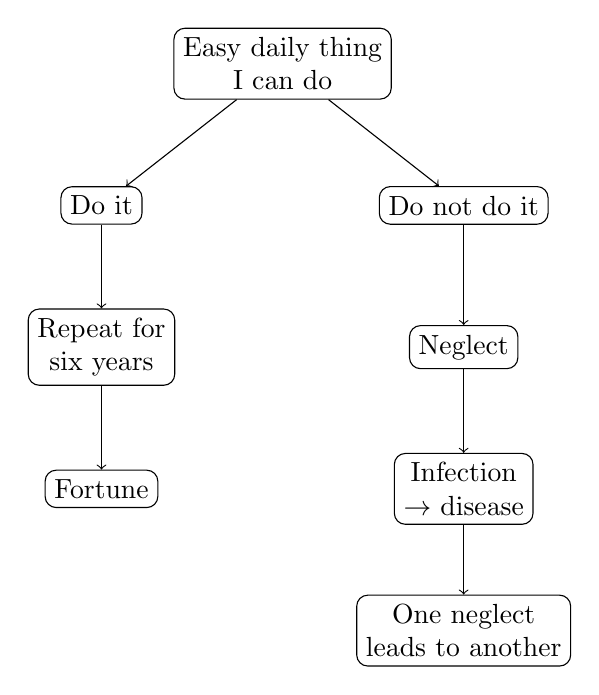
\begin{tikzpicture}
\node[draw, rounded corners, align=center] (top) at (0,0) {Easy daily thing\\I can do};

\node[draw, rounded corners, align=center] (left1) at (-2.3,-1.8) {Do it};
\node[draw, rounded corners, align=center] (left2) at (-2.3,-3.6) {Repeat for\\six years};
\node[draw, rounded corners, align=center] (left3) at (-2.3,-5.4) {Fortune};

\node[draw, rounded corners, align=center] (right1) at (2.3,-1.8) {Do not do it};
\node[draw, rounded corners, align=center] (right2) at (2.3,-3.6) {Neglect};
\node[draw, rounded corners, align=center] (right3) at (2.3,-5.4) {Infection\\$\to$ disease};
\node[draw, rounded corners, align=center] (right4) at (2.3,-7.2) {One neglect\\leads to another};

\draw[->] (top) -- (left1);
\draw[->] (left1) -- (left2);
\draw[->] (left2) -- (left3);

\draw[->] (top) -- (right1);
\draw[->] (right1) -- (right2);
\draw[->] (right2) -- (right3);
\draw[->] (right3) -- (right4);
\end{tikzpicture}
\caption{Transcript-derived decision structure: the same easy act can be done or neglected, and the two accumulations diverge.}
\end{figure}

Rohn then states the practical form of the negative accumulation:
\begin{equation}
\text{Should do it}+\text{Could do it}+\text{Don't do it}
\Longrightarrow
\text{formula for disaster}.
\end{equation}

And the long-time version is just as clear:
\begin{equation}
\text{Six years of accumulated neglect}
\Longrightarrow
\text{undesired life, work, possessions, and self}.
\end{equation}

By this point we can see why the lecture had to move in the order it did. Environment first, then openings, then instruction, then self-change, then definition, and only at the end the full arithmetic of neglect.

\section{Summary}

The lecture begins with a provocative word and spends the rest of its time earning it. First we are given three reasons: America, opportunity, teacher. Then the teacher's method fixes the outside world and varies the self. From there the audience is warned that the next six years will resemble the last unless the decisive variable changes. The ``not much list'' strips away external rescue. Shoaff's promise relocates power inside, beginning with philosophy. The sailing metaphor sharpens the same point. Only then does the lecture return to ``easy'' and define it in a way compatible with hard work. At the end, success and failure are distinguished by one thing only: whether we neglect the easy acts we could have done.

The two shortest relations in the lecture remain the strongest:
\begin{equation}
\text{If you change} \Longrightarrow \text{everything changes for you},
\end{equation}
and
\begin{equation}
\text{Changed life} \Longleftarrow \text{it was me}.
\end{equation}

That is the full movement of the chapter: favorable field, repeatable opportunity, instruction, fixed outside, changed self, and then the long accumulation of disciplined non-neglect.